\chapter{Fundamentação teórica}

\section{Concorrentes no mercado}
%Realizar controle de estoque e elaborar orçamentos utilizando estes como base, não chega a ser uma novidade, existe no mercado diversos softwares que realizam esta atividade para os mais variados segmentos, incluindo paisagismo, floricultura e jardinagem. 

Existem diversos \textit{softwares} no mercado que realizam o controle de estoque e a elaboração de orçamentos para os mais variados segmentos, incluindo paisagismo, floricultura e jardinagem.
Entretanto, estes sistemas costumam ser genéricos, de difícil manipulação por parte dos usuários, devido a interfaces pesadas e com muita informação que dificultam e desencorajam sua utilização.

%Existem também sistemas específicos para cada tarefa (Orçamento, estoque, clientes etc...), mas seus custos de aquisição também impossibilitam sua utilização. 
Existem também sistemas específicos para cada tarefa (orçamento, estoque, clientes, entre outros...), mas os custos de aquisição inviabilizam os comerciantes de adquirirem tal sistemas. 
A seguir constam 2 sistemas que possuem funcionalidades similares ao proposto neste trabalho cada qual com suas características, pontos fortes e fracos. 

\subsection{AuE CalcLANDSCAPE}

\begin{figure}[htp]
\centering
\caption{Logotipo do AuE CalcLandscape}

\includegraphics[width=4cm]{imagens/lands.png}
\fonte{Adaptado de \cite{aue}}
\label{fig:logoAueCalc}
\end{figure}


O CalcLandscape conforme a Figura \ref{fig:logoAueCalc} é uma ferramenta voltada para criação de orçamentos com base em projetos de paisagismo e projetos de irrigação, desenvolvida pela empresa AuE Software. O sistema faz parte de um pacote de \textit{softwares} que visam auxiliar o processo de desenvolvimento de projetos de paisagismo, desde a fase de elaboração de projetos, através dos \textit{softwares} AutoLandscape e HydroLandscape, até sua fase final com emissão de orçamentos detalhados. 

Características: sistema especialmente voltado para projetos de paisagismo.
O \textit{software} pode elaborar orçamentos de jardins com base em projetos de paisagismo e projetos de irrigação.  As telas de elaboração e geração de orçamentos podem ser vistas nas Figuras \ref{fig:aueTelaElaboraçãoOrçamento} e \ref{fig:aueorcamentoAue}, respectivamente. O \textit{software} também conta com um catálogo próprio com uma vasta quantidade de itens cadastrados \cite{aue}.

\begin{figure}[htp]
\centering
\caption{Tela de elaboração orçamentos}
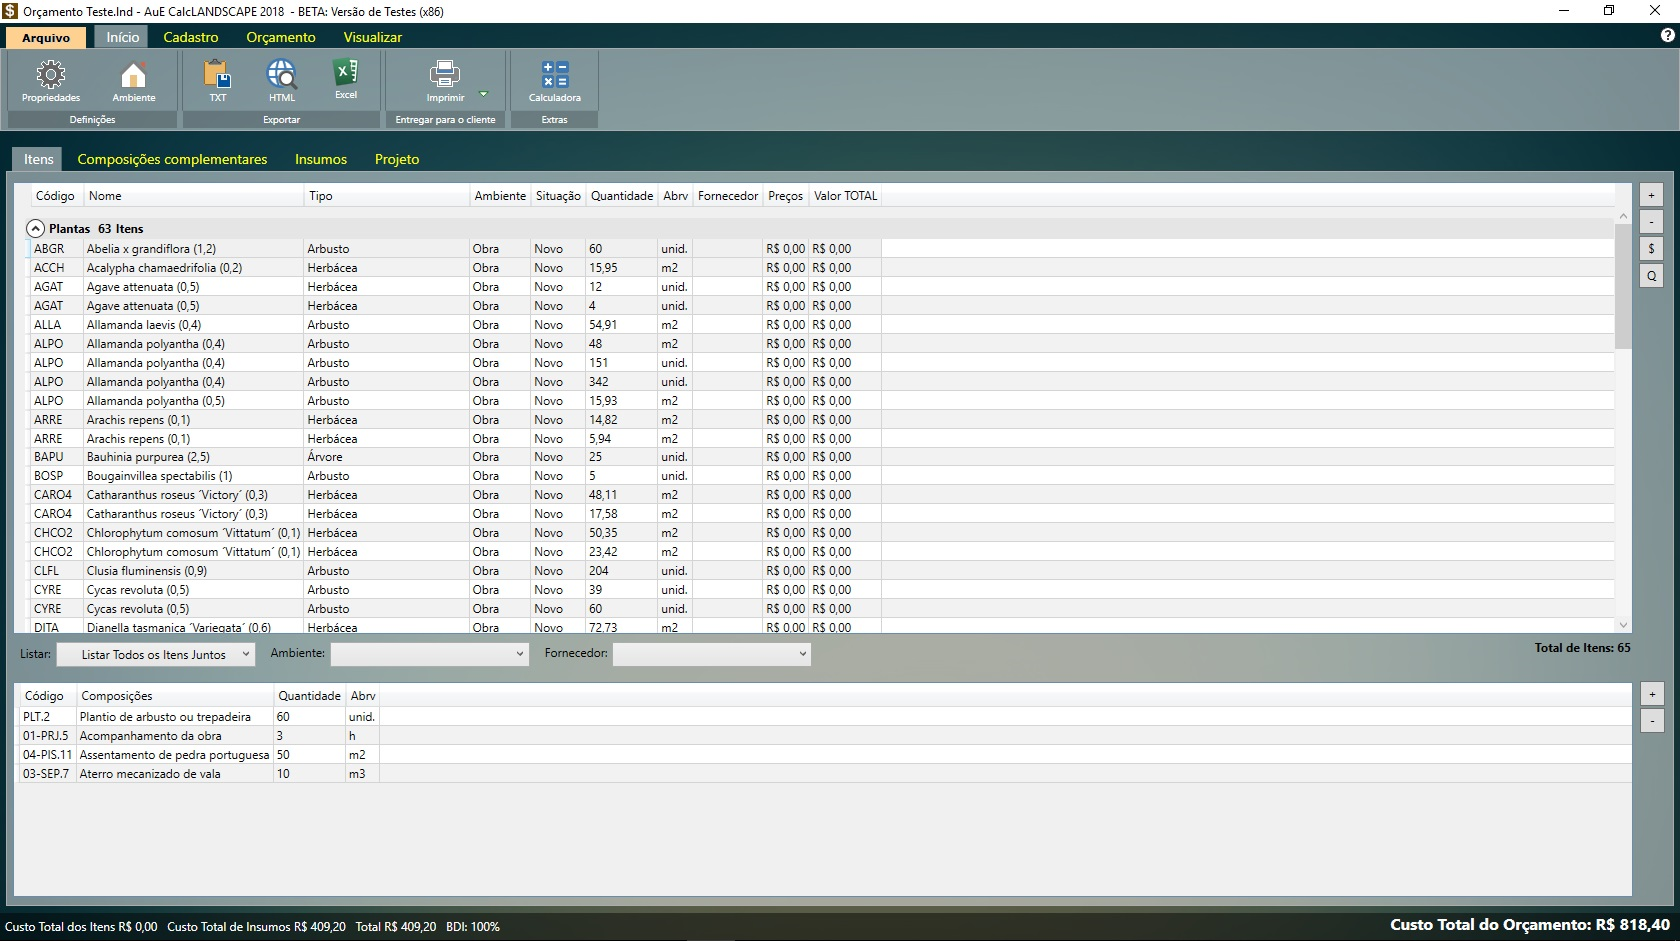
\includegraphics[width=13cm]{imagens/ElaOrcAUE.png}
\label{fig:aueTelaElaboraçãoOrçamento}
\fonte{Aue Software \cite{aue}.}
\end{figure}

 \begin{figure}[htp]
\centering
\caption{Orçamento gerado pelo sistema}
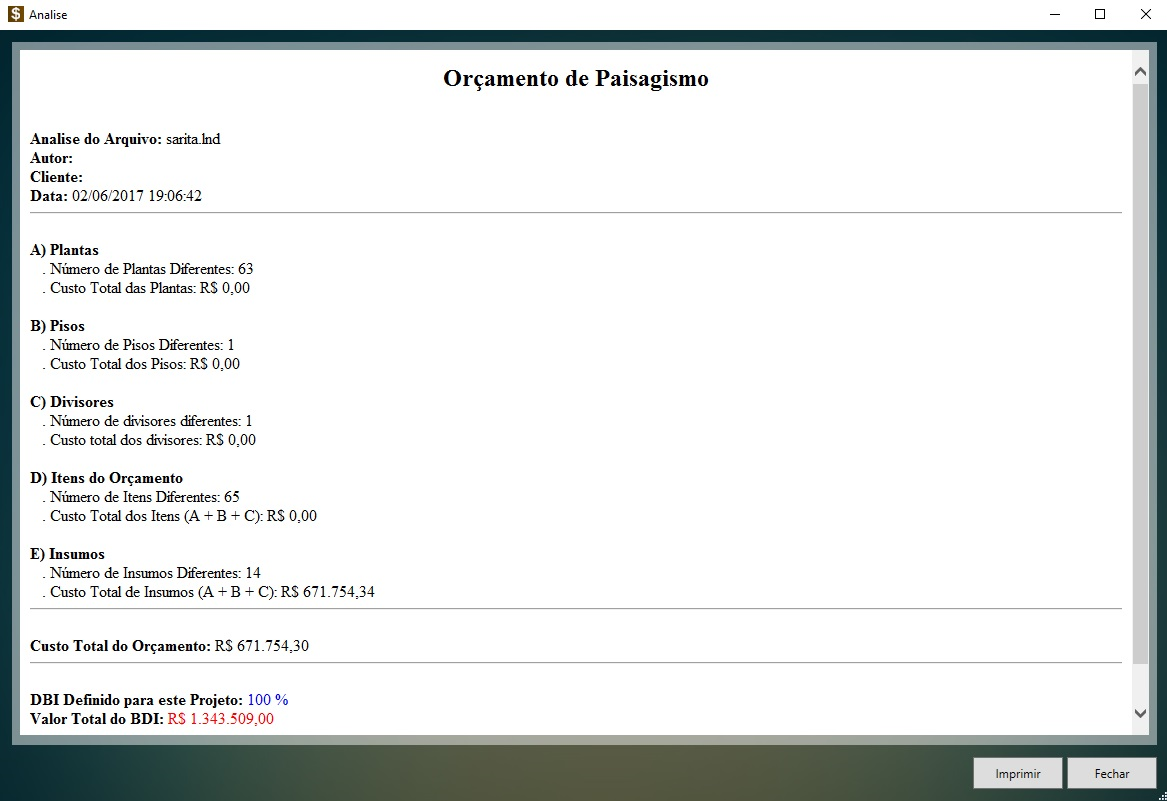
\includegraphics[width=13cm]{imagens/OrcAUE.png}
\label{fig:aueorcamentoAue}
\fonte{Aue Software \cite{aue}.}
\end{figure}

Pontos fortes:
\begin{itemize}
\item Banco de dados flexível: permite cadastrar novos itens.
 \item Desenvolvido especificamente para projetos de paisagismo e jardinagem.
 \item Banco de dados com muitos itens cadastrados.
 \end{itemize}
 
Pontos fracos:
\begin{itemize}
    \item Interface pesada que desencoraja a interação entre usuário-computador.
    \item O usuário deve possuir outros sistemas do grupo, pois funciona de forma integrada.
    \item Custo de licença individual.
 \end{itemize}
 
%Custo aproximados: 2200,00


\subsection{MarketUP}

A MarketUP, Figura \ref{fig:logoMarketUP}, é uma ferramenta que busca auxiliar no gerenciamento de empresas de vários segmentos comerciais. Fornece serviços como controle de estoque (Figura \ref{fig:ControleEstoqueMarketUP}), cadastro de produtos (Figura \ref{fig:CadastroProdutoMarketUP}), entre outros. 

\begin{figure}[htp]
\centering
\caption{Logo MarketUP}

\includegraphics[width=8cm]{imagens/mark.png}
\fonte{Site oficial - MarketUP}
\label{fig:logoMarketUP}
\end{figure}


Características: sistema completo de gestão grátis e online. Fornece diversos módulos para realizar o controle de toda empresa, incluindo: gestão financeira, vendas, clientes, compra e estoque. Além de emitir relatórios gerenciais e notas fiscais. É desenvolvido para empresas dos mais diversos segmentos \cite{marketup}.

\begin{figure}[htp]
\centering
\caption{Tela de controle de estoque}
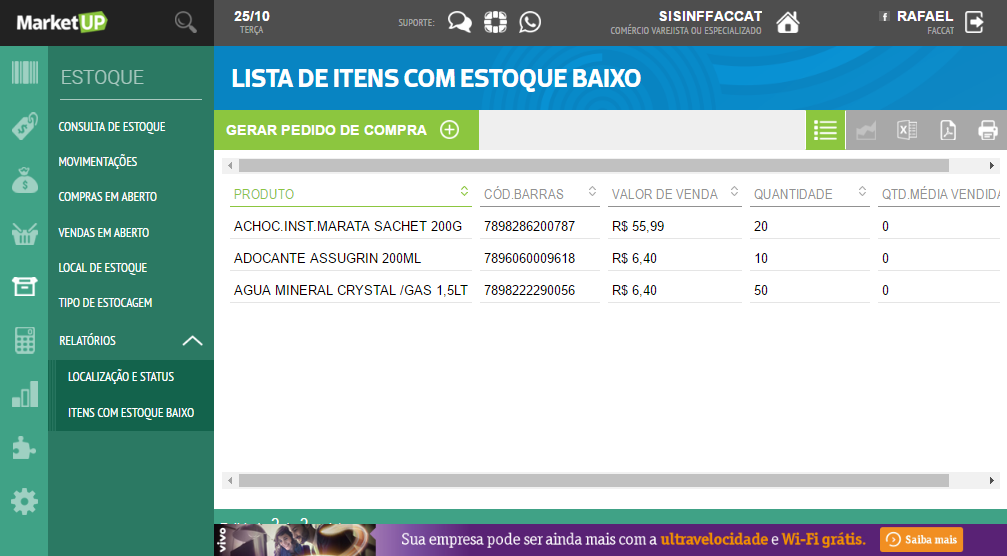
\includegraphics[width=15cm]{imagens/estoque-MarktUP.png}
\label{fig:ControleEstoqueMarketUP}
\fonte{MarketUP \cite{marketup}}
\end{figure}

\begin{figure}[htp]
\centering
\caption{Tela cadastro de produtos}
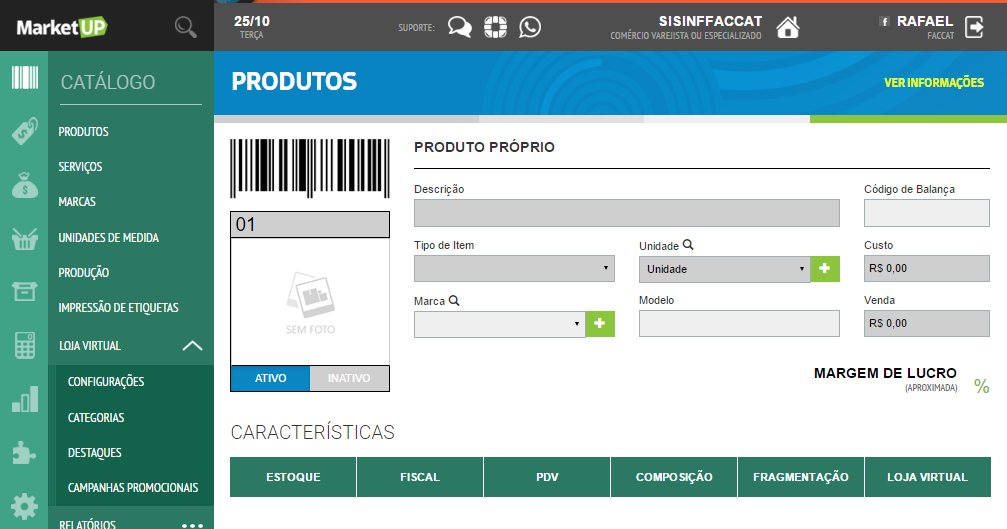
\includegraphics[width=16cm]{imagens/CadProdMark.png}
\label{fig:CadastroProdutoMarketUP}
%\fonte{Site oficial - MarketUP}
\fonte{MarketUP \cite{marketup}}
\end{figure}


Pontos fortes: 
\begin{itemize}
            \item Sistema de gestão completo.
            \item Totalmente grátis.
            \item Emite nota fiscal.
            \item Interface gráfica de fácil interação.
 \end{itemize}
                
Pontos fracos: 
\begin{itemize}
    \item Necessário ter acesso a internet .
    \item Sistema genérico, pois atende vários segmentos.
    \item Lentidão para realizar algumas operações.
\end{itemize}
            
